\section{Acteurs}
%%%%%%%%%%%%%%%%%%%%%
L'appellation "acteurs du jeu" d�signe :
\begin{itemize}
\item �l�ve lyc�en (Terminale S SVT)
\item �l�ve coll�gien (Biologie)
\end{itemize}

\section{Besoins du client}
%%%%%%%%%%%%%%%%%%%%%%%%%%%%%%%
Nous avons besoin de d�velopper une application qui permette de s'initier - sans aucune notion particuli�re - au fonctionnement du syst�me immunitaire dans le corps humain.
\\
\\
De m�me pour les utilisateurs avanc�s, le jeu doit permettre d'aller plus loin dans l'apprentissage.
\begin{itemize}
\item lancer le jeu
\item apprendre � combattre une infection bact�riologique
\item apprendre � combattre un virus
\item aller plus loin dans l'apprentissage
\end{itemize}

\section{R�cits d'utilisation}
%%%%%%%%%%%%%%%%%%%%%%%%%%%%%%%%%%
\subsection{RU 01 : lancement du jeu}
{\bf En tant que} joueur
{\bf je souhaite} pouvoir lancer le jeu
{\bf afin d'} apprendre le fonctionnement du syst�me immunitaire humain - tout en m'amusant.

\subsection{RU 02 : combat contre une bact�rie}
{\bf En tant que} joueur
{\bf je souhaite} pouvoir combattre une bact�rie
{\bf afin de} comprendre la r�action sp�cifique du corps face � une bact�rie.

\subsection{RU 03 : combat contre un virus}
{\bf En tant que} joueur
{\bf je souhaite} pouvoir combattre un virus
{\bf afin de} comprendre la r�action sp�cifique du corps face � un virus.

\subsection{RU 04 : obtenir des informations}
{\bf En tant que} joueur
{\bf je souhaite} pouvoir obtenir des informations d�taill�es � propos d'un agent pathog�ne.
{\bf afin d'}aller plus loin dans mon apprentissage

\section{Rappels des fonctionnalit�s}
\begin{itemize}
	\item lancer le jeu
	\item configurer le son
	\item s�lectionner un niveau
	\item lancer la partie
	\item acc�der aux fiches information
\end{itemize}

\section{Sc�nario d'utilisation}

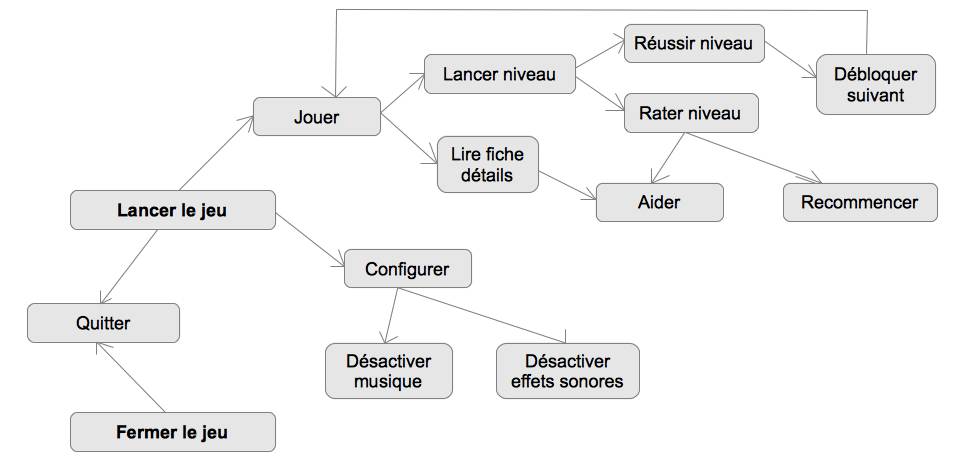
\includegraphics[scale=0.4]{Images/scenario.jpg}

\section{Contraintes}
Nous allons devoir g�rer les types d'agents pathog�nes � combattre. En effet, selon que ceux-ci soient des virus ou des bact�ries, la marche � suivre pour les �liminer n'est pas la m�me.
\\
\\
Les m�canismes biologiques en jeu sont diff�rents mais font intervenir les m�mes acteurs. Il faudra donc adapter leur comportement - et la r�action du jeu qui y est associ�e - en fonction de l'ennemi combattu.
Le jeu sera d'abord d�velopp� pour le combat contre des bact�ries, techniquement plus simple � mettre en oeuvre.